\subsection{Independent-unit repetition: current completion}
\label{sec:independent-repetition-status}
The repetition manifest targets five complete units. At this reporting checkpoint, 5 of five units have complete main analyses.
The following are unit-level observations. The 32 conditions and their candidate pairs within each unit are dependent measurements, and are not pooled as binomial trials.
\begin{center}\small
\begin{tabular}{lrrrr}
Unit & A: $B_t>0$ & A: $\Delta>0$ & B: above mean & B: unique first\\\hline
archdev001 & 26/32 & 18/32 & 29/32 & 19/32\\
unit02 & 28/32 & 18/32 & 30/32 & 18/32\\
unit03 & 29/32 & 18/32 & 30/32 & 17/32\\
unit04 & 28/32 & 18/32 & 30/32 & 20/32\\
unit05 & 26/32 & 18/32 & 29/32 & 18/32\\
\end{tabular}\end{center}
The companion results retain unrounded condition effects, unit-level sample standard deviations and ranges, all unit-specific values, undefined cells, and direction consistency. A sign change near zero is interpreted with its magnitude rather than as evidence of a substantive reversal.
These repetitions jointly change sampling, shared architecture-level initialization, batch order, and the registered training random streams. They do not isolate the contribution of each random factor, and they do not test specialists initialized independently within a unit.
\paragraph{Four new repetitions, excluding the exploratory unit.}
All four newly registered units have complete main analyses. They are presented first, without the historical exploratory unit. Each primary count retains its denominator of 32 dependent conditions, and each summary observation is a complete unit.
\begin{center}\small\begin{tabular}{lrrrr}\toprule
Statistic & Mean & Sample SD & Minimum & Maximum\\\midrule
A: $B_t>0$ & 27.750000 & 1.258306 & 26.000000 & 29.000000\\
A: $\Delta>0$ & 18.000000 & 0.000000 & 18.000000 & 18.000000\\
B: above other mean & 29.750000 & 0.500000 & 29.000000 & 30.000000\\
B: unique first & 18.250000 & 1.258306 & 17.000000 & 20.000000\\
\bottomrule\end{tabular}\end{center}
The new-only exact sign agreement is reported separately below; agreement does not imply a practically large effect.
\begin{center}\small\begin{tabular}{lrrrr}\toprule
Effect & Positive in all 4 & Negative in all 4 & Mixed or zero & Undefined unit(s)\\\midrule
A: $B_t$ & 24 & 2 & 6 & 0\\
A: $\Delta$ & 18 & 14 & 0 & 0\\
B: trained contrast & 27 & 1 & 4 & 0\\
\bottomrule\end{tabular}\end{center}
\paragraph{All five units, including the historical exploratory unit.}
The combined description adds the original exploratory unit to the same four new repetitions. These overlapping cohorts are not independent groups, and the historical unit is not counted as a new replication.
\begin{center}\small\begin{tabular}{lrrrr}\toprule
Statistic & Mean & Sample SD & Minimum & Maximum\\\midrule
A: $B_t>0$ & 27.400000 & 1.341641 & 26.000000 & 29.000000\\
A: $\Delta>0$ & 18.000000 & 0.000000 & 18.000000 & 18.000000\\
B: above other mean & 29.600000 & 0.547723 & 29.000000 & 30.000000\\
B: unique first & 18.400000 & 1.140175 & 17.000000 & 20.000000\\
\bottomrule\end{tabular}\end{center}
The combined sign summary again uses the original exact zero boundary; a near-zero sign change is not described as a substantive reversal.
\begin{center}\small\begin{tabular}{lrrrr}\toprule
Effect & Positive in all 5 & Negative in all 5 & Mixed or zero & Undefined unit(s)\\\midrule
A: $B_t$ & 24 & 2 & 6 & 0\\
A: $\Delta$ & 18 & 14 & 0 & 0\\
B: trained contrast & 27 & 1 & 4 & 0\\
\bottomrule\end{tabular}\end{center}
The repetitions jointly resample data, shared architecture-level initialization, batch order, and registered training streams. They do not isolate these factors, test independently initialized task specialists within a unit, or identify a mathematical mechanism. Neither the conditions nor pooled positive counts are independent binomial trials.
Figure~\ref{fig:independent-repetition} shows every unit's primary continuous effects. The following tables report all 32 conditions for each effect across all five units; six-decimal formatting is display-only. Separate new-four and all-five condition-effect and unit-count CSV files retain unrounded summaries, all unit-specific values, and finite-unit counts.
\begin{figure}[p]\centering
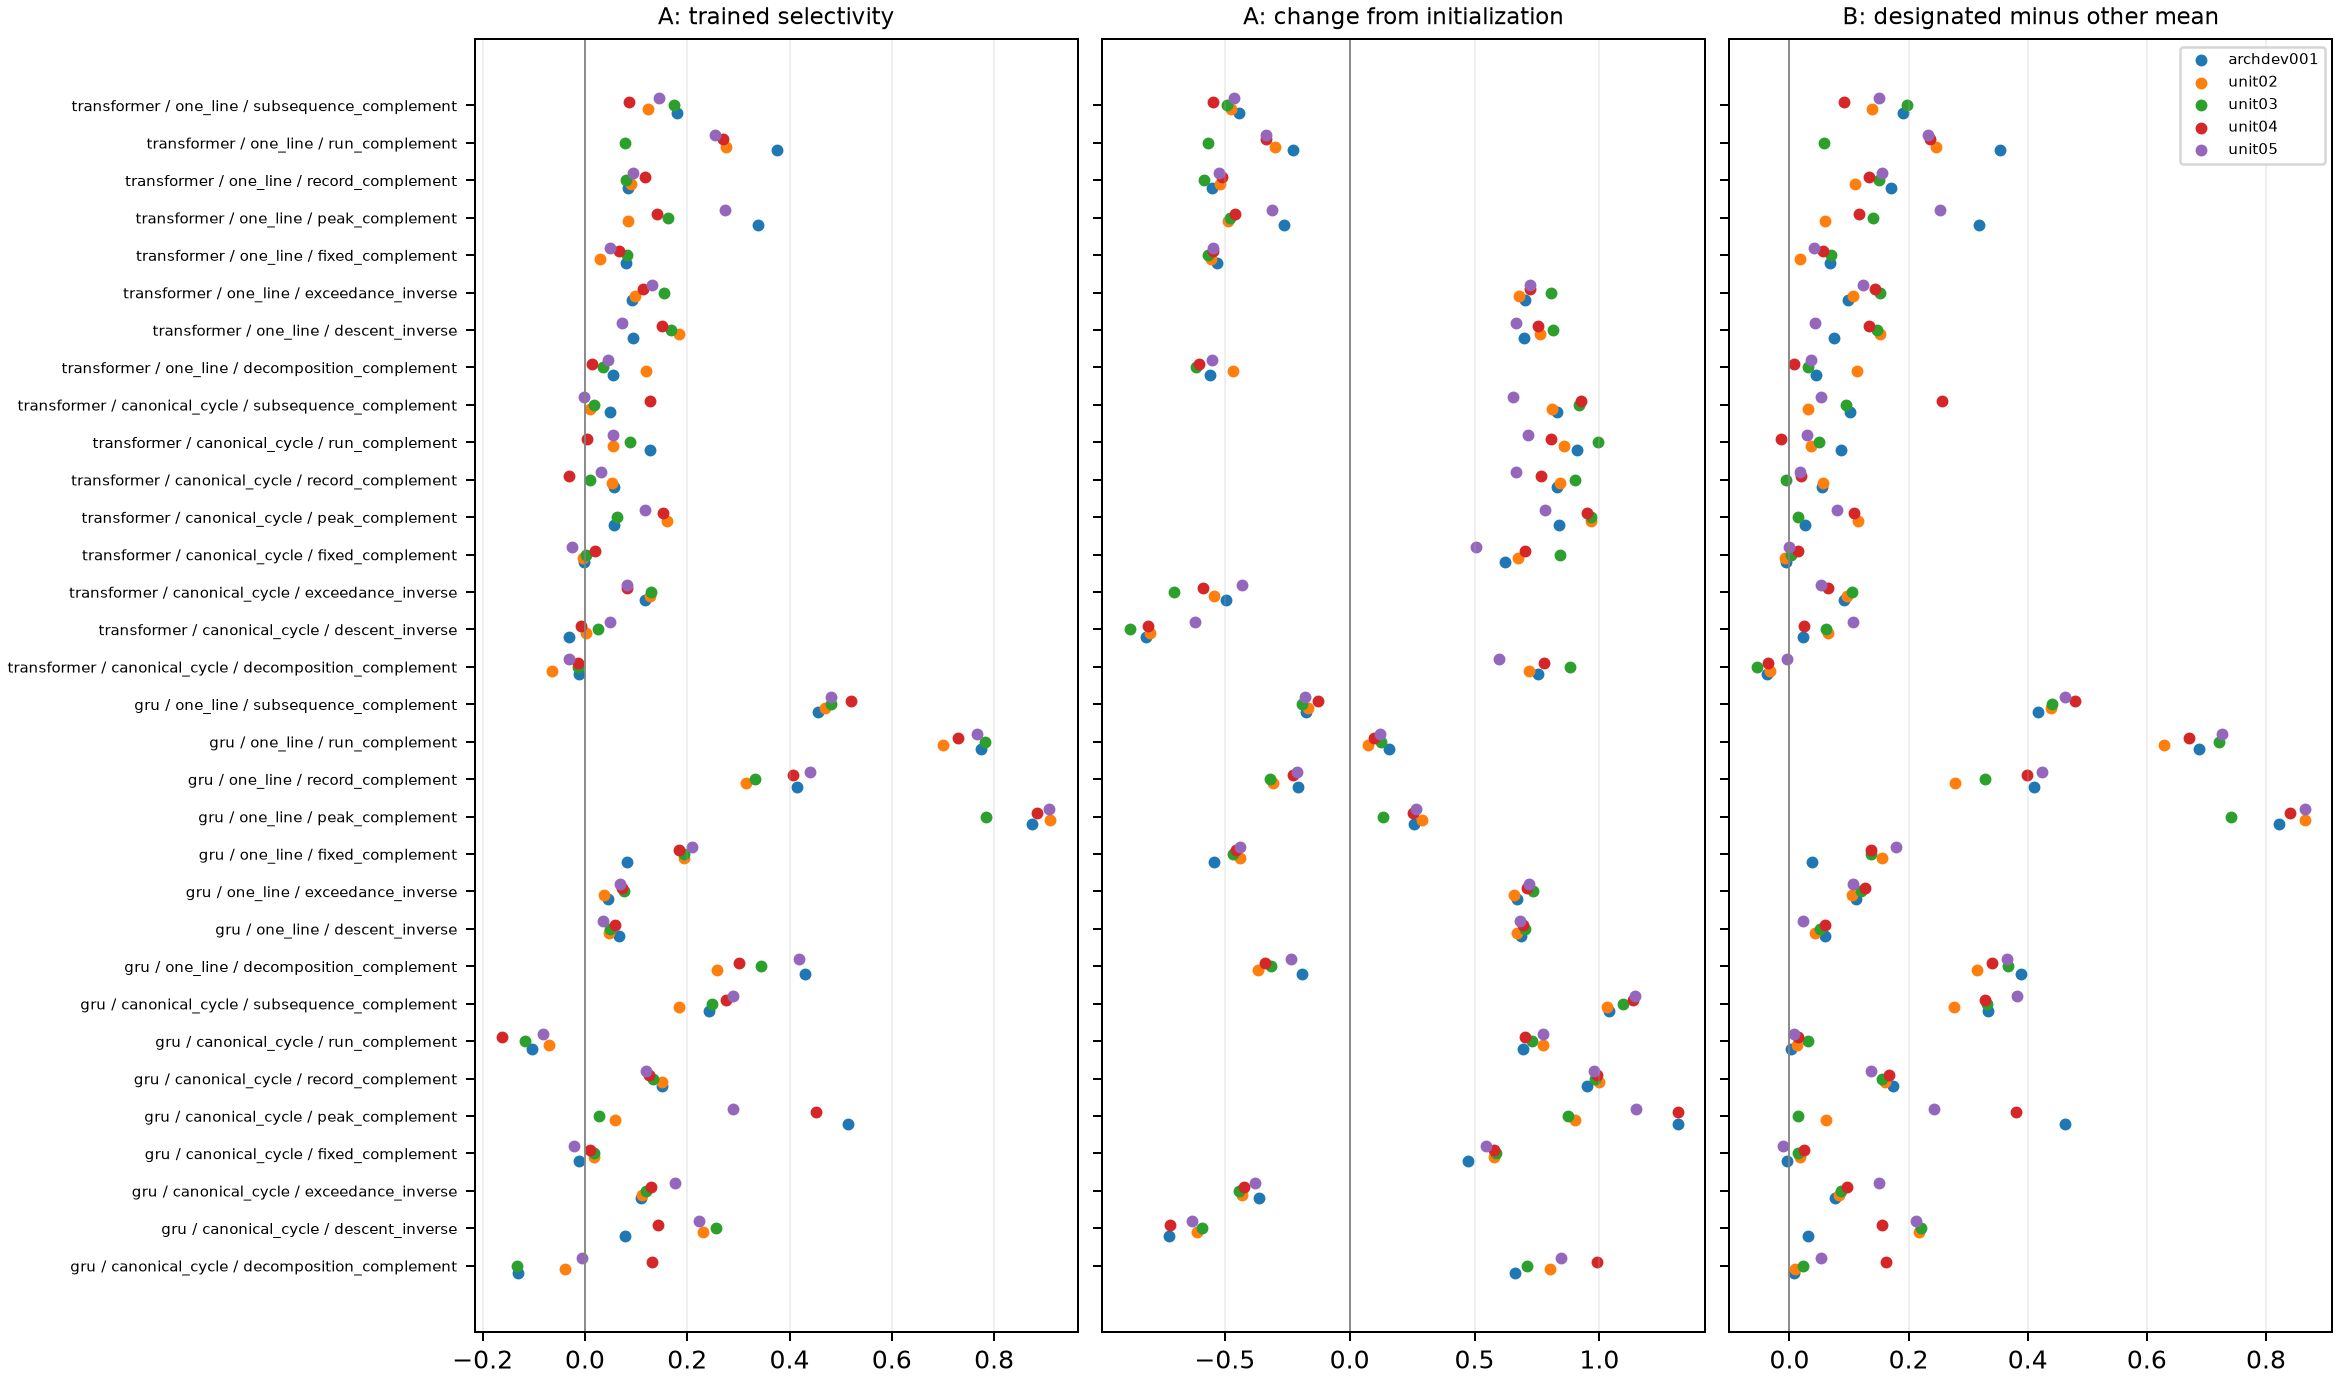
\includegraphics[width=\textwidth]{figures/figure6_independent_repetition.png}
\caption{All registered units' answer-controlled final-layer ordinary-CKA effects. Each marker is a unit-specific measurement of a dependent condition; no condition-level independence or practical-effect threshold is assumed.}\label{fig:independent-repetition}\end{figure}
\begin{table}[p]\centering\scriptsize
\begin{tabular}{llrrrrr}\toprule
Config./encoding & Relation & Finite units & Mean & Sample SD & Minimum & Maximum\\\midrule
GRU/cycle & decomposition\_complement & 5 & -0.035552 & 0.108425 & -0.132320 & 0.130549\\
GRU/cycle & descent\_inverse & 5 & 0.186680 & 0.073480 & 0.079276 & 0.256132\\
GRU/cycle & exceedance\_inverse & 5 & 0.129090 & 0.027690 & 0.109796 & 0.176690\\
GRU/cycle & fixed\_complement & 5 & 0.002117 & 0.017705 & -0.021377 & 0.016971\\
GRU/cycle & peak\_complement & 5 & 0.268525 & 0.221656 & 0.027056 & 0.514493\\
GRU/cycle & record\_complement & 5 & 0.136079 & 0.014122 & 0.120187 & 0.150822\\
GRU/cycle & run\_complement & 5 & -0.107199 & 0.035533 & -0.161865 & -0.070777\\
GRU/cycle & subsequence\_complement & 5 & 0.248385 & 0.040646 & 0.184627 & 0.290293\\
GRU/line & decomposition\_complement & 5 & 0.350332 & 0.073850 & 0.258553 & 0.429695\\
GRU/line & descent\_inverse & 5 & 0.051791 & 0.012157 & 0.035430 & 0.067502\\
GRU/line & exceedance\_inverse & 5 & 0.060323 & 0.017453 & 0.038073 & 0.076995\\
GRU/line & fixed\_complement & 5 & 0.173021 & 0.051357 & 0.082685 & 0.210251\\
GRU/line & peak\_complement & 5 & 0.871637 & 0.051620 & 0.783431 & 0.909916\\
GRU/line & record\_complement & 5 & 0.381370 & 0.054580 & 0.314784 & 0.439699\\
GRU/line & run\_complement & 5 & 0.750349 & 0.034896 & 0.699258 & 0.782085\\
GRU/line & subsequence\_complement & 5 & 0.481408 & 0.024476 & 0.454861 & 0.520913\\
TF/cycle & decomposition\_complement & 5 & -0.026939 & 0.022494 & -0.064317 & -0.012266\\
TF/cycle & descent\_inverse & 5 & 0.007627 & 0.031143 & -0.032044 & 0.049563\\
TF/cycle & exceedance\_inverse & 5 & 0.107307 & 0.023779 & 0.081727 & 0.129423\\
TF/cycle & fixed\_complement & 5 & -0.001416 & 0.015829 & -0.024654 & 0.019520\\
TF/cycle & peak\_complement & 5 & 0.109944 & 0.048769 & 0.056991 & 0.160157\\
TF/cycle & record\_complement & 5 & 0.023970 & 0.035828 & -0.030363 & 0.056211\\
TF/cycle & run\_complement & 5 & 0.065625 & 0.045578 & 0.004492 & 0.127034\\
TF/cycle & subsequence\_complement & 5 & 0.039989 & 0.052007 & -0.002588 & 0.126454\\
TF/line & decomposition\_complement & 5 & 0.053391 & 0.040125 & 0.012897 & 0.119763\\
TF/line & descent\_inverse & 5 & 0.133686 & 0.048226 & 0.073049 & 0.183499\\
TF/line & exceedance\_inverse & 5 & 0.117723 & 0.025838 & 0.091672 & 0.155296\\
TF/line & fixed\_complement & 5 & 0.061053 & 0.022703 & 0.028541 & 0.082682\\
TF/line & peak\_complement & 5 & 0.200002 & 0.103834 & 0.083668 & 0.338195\\
TF/line & record\_complement & 5 & 0.092879 & 0.014408 & 0.080943 & 0.117189\\
TF/line & run\_complement & 5 & 0.250521 & 0.107848 & 0.077730 & 0.375633\\
TF/line & subsequence\_complement & 5 & 0.141615 & 0.039031 & 0.085268 & 0.179907\\
\bottomrule\end{tabular}
\caption{Comparison A: trained selectivity $B_t$; all fixed conditions. Statistics describe finite complete-unit observations; undefined values are not filled with zero.}
\label{tab:independent-effect-1}\end{table}
\begin{table}[p]\centering\scriptsize
\begin{tabular}{llrrrrr}\toprule
Config./encoding & Relation & Finite units & Mean & Sample SD & Minimum & Maximum\\\midrule
GRU/cycle & decomposition\_complement & 5 & 0.801675 & 0.127590 & 0.661883 & 0.989008\\
GRU/cycle & descent\_inverse & 5 & -0.655743 & 0.061643 & -0.721681 & -0.590702\\
GRU/cycle & exceedance\_inverse & 5 & -0.407989 & 0.035334 & -0.444044 & -0.361238\\
GRU/cycle & fixed\_complement & 5 & 0.552587 & 0.046222 & 0.475427 & 0.587825\\
GRU/cycle & peak\_complement & 5 & 1.110420 & 0.213311 & 0.875301 & 1.313732\\
GRU/cycle & record\_complement & 5 & 0.979674 & 0.018758 & 0.949758 & 0.998424\\
GRU/cycle & run\_complement & 5 & 0.734606 & 0.037090 & 0.696079 & 0.773275\\
GRU/cycle & subsequence\_complement & 5 & 1.087612 & 0.053612 & 1.028659 & 1.142926\\
GRU/line & decomposition\_complement & 5 & -0.288687 & 0.074555 & -0.368379 & -0.190155\\
GRU/line & descent\_inverse & 5 & 0.686963 & 0.011985 & 0.672121 & 0.703084\\
GRU/line & exceedance\_inverse & 5 & 0.698427 & 0.033387 & 0.658614 & 0.736014\\
GRU/line & fixed\_complement & 5 & -0.468261 & 0.042676 & -0.541572 & -0.438145\\
GRU/line & peak\_complement & 5 & 0.239748 & 0.060585 & 0.134395 & 0.289020\\
GRU/line & record\_complement & 5 & -0.253974 & 0.054697 & -0.319829 & -0.205284\\
GRU/line & run\_complement & 5 & 0.114432 & 0.031683 & 0.072815 & 0.156065\\
GRU/line & subsequence\_complement & 5 & -0.168197 & 0.025528 & -0.190877 & -0.124884\\
TF/cycle & decomposition\_complement & 5 & 0.745435 & 0.103206 & 0.597633 & 0.882883\\
TF/cycle & descent\_inverse & 5 & -0.784519 & 0.098964 & -0.881520 & -0.617322\\
TF/cycle & exceedance\_inverse & 5 & -0.552511 & 0.102565 & -0.704416 & -0.432954\\
TF/cycle & fixed\_complement & 5 & 0.668531 & 0.123647 & 0.504442 & 0.844074\\
TF/cycle & peak\_complement & 5 & 0.900735 & 0.085329 & 0.782472 & 0.967102\\
TF/cycle & record\_complement & 5 & 0.802147 & 0.089541 & 0.667241 & 0.903763\\
TF/cycle & run\_complement & 5 & 0.857045 & 0.106075 & 0.714481 & 0.995272\\
TF/cycle & subsequence\_complement & 5 & 0.827241 & 0.108881 & 0.655895 & 0.924758\\
TF/line & decomposition\_complement & 5 & -0.560533 & 0.058449 & -0.616042 & -0.468138\\
TF/line & descent\_inverse & 5 & 0.738918 & 0.058852 & 0.664186 & 0.815101\\
TF/line & exceedance\_inverse & 5 & 0.726243 & 0.047893 & 0.677631 & 0.804868\\
TF/line & fixed\_complement & 5 & -0.549669 & 0.013471 & -0.568796 & -0.531440\\
TF/line & peak\_complement & 5 & -0.399472 & 0.104539 & -0.486965 & -0.262120\\
TF/line & record\_complement & 5 & -0.537138 & 0.030343 & -0.584051 & -0.510372\\
TF/line & run\_complement & 5 & -0.352782 & 0.127817 & -0.567183 & -0.226384\\
TF/line & subsequence\_complement & 5 & -0.483321 & 0.038961 & -0.545673 & -0.441963\\
\bottomrule\end{tabular}
\caption{Comparison A: initialization-relative change $\Delta$; all fixed conditions. Statistics describe finite complete-unit observations; undefined values are not filled with zero.}
\label{tab:independent-effect-2}\end{table}
\begin{table}[p]\centering\scriptsize
\begin{tabular}{llrrrrr}\toprule
Config./encoding & Relation & Finite units & Mean & Sample SD & Minimum & Maximum\\\midrule
GRU/cycle & decomposition\_complement & 5 & 0.050654 & 0.064517 & 0.007581 & 0.161320\\
GRU/cycle & descent\_inverse & 5 & 0.167397 & 0.080715 & 0.031018 & 0.220184\\
GRU/cycle & exceedance\_inverse & 5 & 0.098286 & 0.029458 & 0.077027 & 0.149573\\
GRU/cycle & fixed\_complement & 5 & 0.008530 & 0.014742 & -0.010370 & 0.024352\\
GRU/cycle & peak\_complement & 5 & 0.232329 & 0.194965 & 0.014029 & 0.462216\\
GRU/cycle & record\_complement & 5 & 0.158416 & 0.014236 & 0.136107 & 0.173730\\
GRU/cycle & run\_complement & 5 & 0.013607 & 0.010796 & 0.002585 & 0.031222\\
GRU/cycle & subsequence\_complement & 5 & 0.329871 & 0.037472 & 0.275388 & 0.381135\\
GRU/line & decomposition\_complement & 5 & 0.355518 & 0.028281 & 0.315268 & 0.388767\\
GRU/line & descent\_inverse & 5 & 0.047141 & 0.015143 & 0.022976 & 0.059501\\
GRU/line & exceedance\_inverse & 5 & 0.113748 & 0.009160 & 0.105238 & 0.126302\\
GRU/line & fixed\_complement & 5 & 0.129463 & 0.053747 & 0.038421 & 0.179057\\
GRU/line & peak\_complement & 5 & 0.827061 & 0.051127 & 0.741708 & 0.865608\\
GRU/line & record\_complement & 5 & 0.367868 & 0.062338 & 0.277790 & 0.424175\\
GRU/line & run\_complement & 5 & 0.686802 & 0.039496 & 0.629292 & 0.725305\\
GRU/line & subsequence\_complement & 5 & 0.447788 & 0.023811 & 0.417526 & 0.479729\\
TF/cycle & decomposition\_complement & 5 & -0.033223 & 0.018079 & -0.054721 & -0.004716\\
TF/cycle & descent\_inverse & 5 & 0.055793 & 0.034539 & 0.022916 & 0.106602\\
TF/cycle & exceedance\_inverse & 5 & 0.082071 & 0.022221 & 0.053247 & 0.104929\\
TF/cycle & fixed\_complement & 5 & 0.000572 & 0.008714 & -0.007220 & 0.014497\\
TF/cycle & peak\_complement & 5 & 0.068600 & 0.046454 & 0.014055 & 0.115062\\
TF/cycle & record\_complement & 5 & 0.028579 & 0.026305 & -0.005070 & 0.056440\\
TF/cycle & run\_complement & 5 & 0.037568 & 0.036290 & -0.014620 & 0.085749\\
TF/cycle & subsequence\_complement & 5 & 0.107628 & 0.088461 & 0.031125 & 0.256887\\
TF/line & decomposition\_complement & 5 & 0.046910 & 0.039611 & 0.008357 & 0.113445\\
TF/line & descent\_inverse & 5 & 0.110450 & 0.048477 & 0.043677 & 0.152716\\
TF/line & exceedance\_inverse & 5 & 0.124917 & 0.023344 & 0.097820 & 0.152517\\
TF/line & fixed\_complement & 5 & 0.050670 & 0.021483 & 0.018126 & 0.070119\\
TF/line & peak\_complement & 5 & 0.177776 & 0.105322 & 0.059873 & 0.318451\\
TF/line & record\_complement & 5 & 0.143816 & 0.023223 & 0.109696 & 0.170685\\
TF/line & run\_complement & 5 & 0.225035 & 0.106071 & 0.057597 & 0.352879\\
TF/line & subsequence\_complement & 5 & 0.153709 & 0.043026 & 0.090895 & 0.197728\\
\bottomrule\end{tabular}
\caption{Comparison B: trained designated-minus-other-mean contrast; all fixed conditions. Statistics describe finite complete-unit observations; undefined values are not filled with zero.}
\label{tab:independent-effect-3}\end{table}

